%\part{Konstruktion}
%\chapter{Programmlogik}

\section{QueryResolution}

\begin{figure}[htb]
    	\centering
  	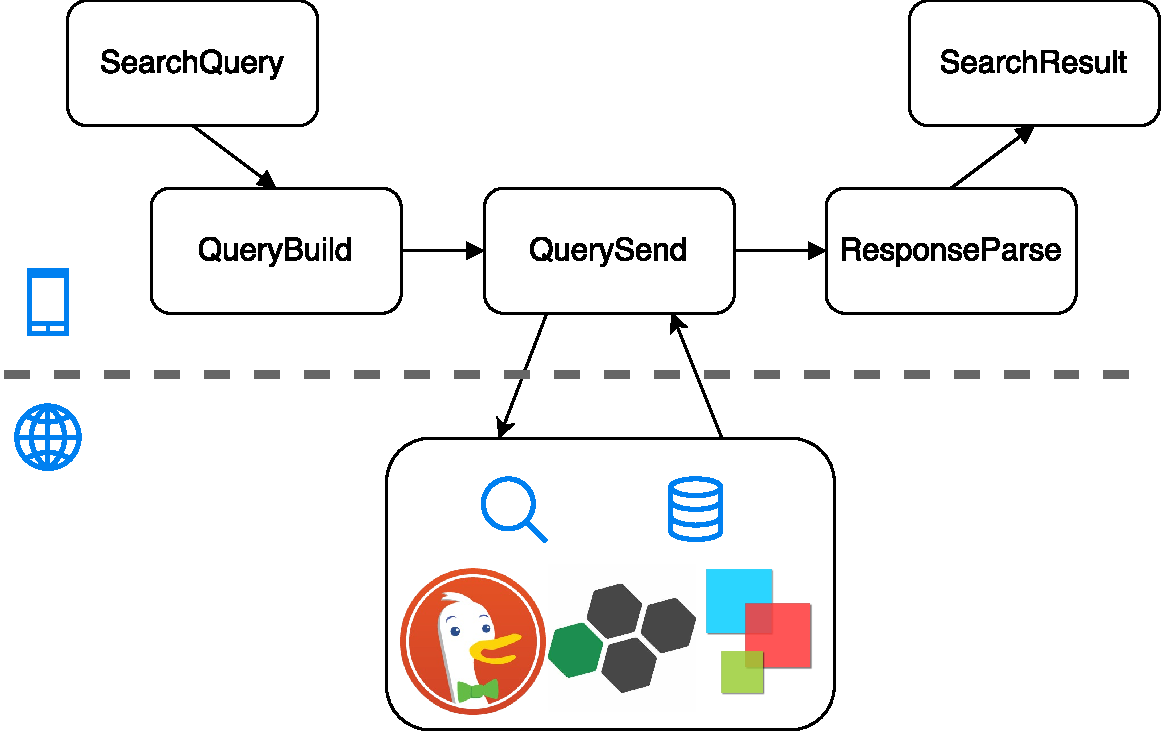
\includegraphics[width=0.6\textwidth]{QueryResolutionOverview}
  	\caption{Übersicht des Moduls QueryResolution}
\end{figure}

\begin{figure}[htb]
    	\centering
  	\includegraphics[width=\textwidth]{QueryResolution}
  	\caption{Aufbau des Moduls QueryResolution}
\end{figure}

%%\part{Konstruktion}
%\chapter{Programmlogik}
%\section{QueryResolution}

\subsection{JSONData}

%\paragraph{Paragraph}
%\subparagraph{Unterparagraph}

%\part{Konstruktion}
%\chapter{Programmlogik}
%\section{QueryResolution}

\subsection{QueryBuild}

Das Modul QueryBuild liefert den größten Teil der Intelligenz im Modul QueryResolution. Die Aufgaben des Moduls sind es, die ConnectionController in QuerySend zu konfigurieren, die Query in das suchmaschinenspezifische Anfrageformat umzuwandeln und dem ConnectionController den Parser für die Antwort zu geben.

Es gibt für jede Suchmaschine eine Implementation der Spezifikation AbstractBuilder, welche durch die Spezifikationen URLAbstractBuilder und JSONAbstractBuilder erweitert wird.

\subsubsection{AbstractBuilder}
\subsubsection{AbstractJSONBuilder}
\subsubsection{AbstractURLBuilder}
\subsubsection{EexcessJSONBuilder}
\subsubsection{FarooURLBuilder}
\subsubsection{DuckDuckGoURLBuilder}
\subsubsection{EEXCESSOrigin}

%\paragraph{Paragraph}
%\subparagraph{Unterparagraph}

%\part{Konstruktion}
%\chapter{Programmlogik}
%\section{QueryResolution}

\subsection{QuerySend}

\begin{figure}[htb]
	\centering
  	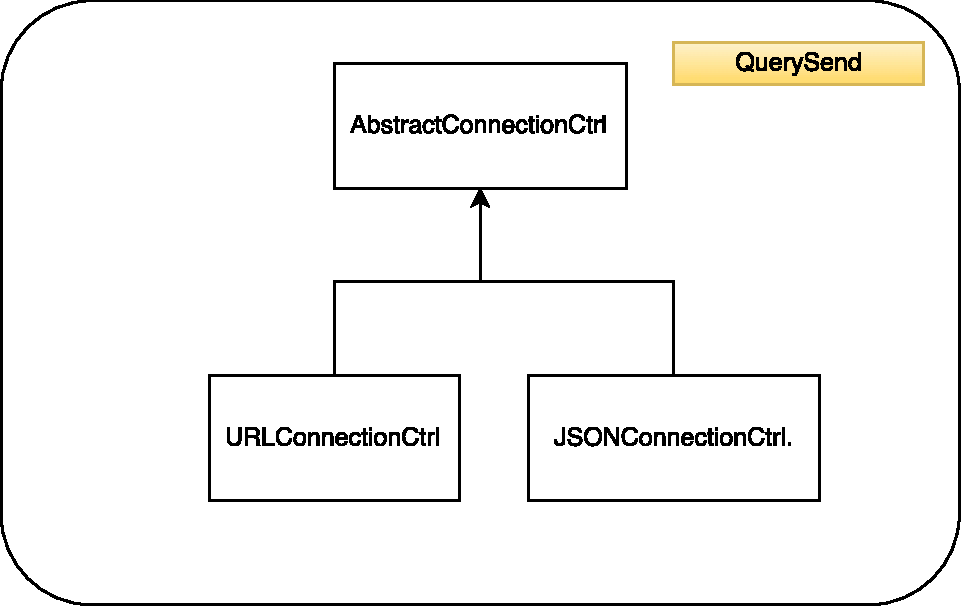
\includegraphics[width=0.8\textwidth]{qr_querysend}
  	\caption{Aufbau des Moduls \lstinline|QuerySend|}
\end{figure}

Im Modul \lstinline|QuerySend| befinden sich die \lstinline|ConnectionController|, die für das Versenden der Anfrage zuständig sind. Sie werden mithilfe von \lstinline|QueryBuild| konfiguriert und erhalten den Parser (\lstinline|ResponseParse|). Vor dem Weiterreichen an den \lstinline|TaskController|, wird durch den Parser noch von NSData zu \lstinline|SearchResult| umgewandelt.
\pagebreak
\clearpage
%\part{Konstruktion}
%\chapter{Programmlogik}
%\section{QueryResolution}

\subsection{ResponseParse}
\begin{figure}[htb]
	\centering
		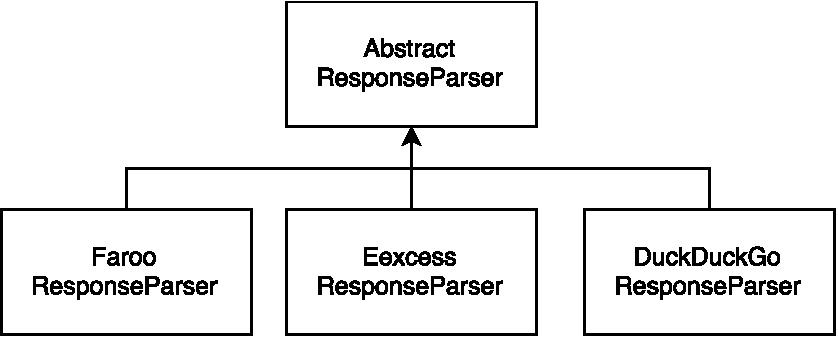
\includegraphics[]{response_parser}
		\caption{Aufbau des Moduls ResponseParse}
		\label{fig:Aufbau des Moduls ResponseParse}
\end{figure}
Der \lstinline|ResponeParser| ist für das Parsen der Antworten der Suchmaschinen in ein allgemeines Format.
Dabei wird in der aktuellen Version zwischen drei Parsern unterschieden.
\subparagraph{FarooResponseParser}
Hier werden die Antworten von Faroo verarbeitet.
\subparagraph{DuckDuckGoResponseParser}
Hier werden die Antworten von DuckDuckGO verarbeitet.
\subparagraph{EexcessResponseParser}
Hier werden die Antworten von Eexcess verarbeitet.
\subparagraph{AbstractResponseParser}
Der \lstinline|AbstractResponseParser| spezifiziert wie die untergeordneten \lstinline|ResponeParser| implementiert werden.

%\paragraph{Paragraph}
%\subparagraph{Unterparagraph}
